% Bagian Analisis Hasil Percobaan
    
\section*{Analisis Hasil Percobaan}
\indent
Pada hari pertama Workshop Telematika peserta diberikan pelajaran mengenai penyolderan dan komponen serta cara untuk implementasinya. Kelompok 17 telah melaksanakan hari pertama dengan menyelesaikan 1 eksperimen, yakni menggunakan 7-segment sebagai komponen utamanya. Kemudian dilanjutkan dengan eksperimen kedua dengan menggunakan Modul LED Chaser kit, kelompok 17 telah melakukan beberapa langkah di eksperimen kedua namun tidak dapat menyelesaikannya hingga berhasil percobaan dikarenakan waktu yang terbatas.

\begin{figure}[H]
    \centering
    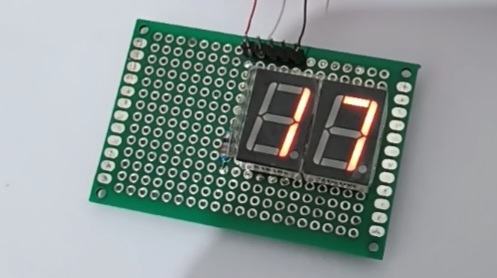
\includegraphics[width=0.2\linewidth]{img/eksperimen_1.jpeg}
    \caption{Gambar Eskperimen 1 Berhasil.} 
    \label{fig:ini2}
\end{figure}

Pada gambar \ref{fig:ini2} dapat menunjukkan bahwa pada percobaan kelompok 17 untuk eksperimen 1 adalah berhasil. Kelompok 17 berhasil menyalakan 7-segment dan membentuk angka kelompoknya yakni angka 17. Berikut adalah alat dan komponen yang Kelompok 17 pakai untuk Workshop hari pertama dan langkah-langkah yang sudah dilalui.
\subsection*{Alat dan Bahan}
\begin{enumerate}
    \item Alat
        \begin{enumerate}[label*=\arabic*.]
            \item Soldering kit
            \item Timah 0.8 mm
            \item Power source
            \item Solder pasta
        \end{enumerate}
    \item Bahan
        \begin{enumerate}[label*=\arabic*.]
            \item PCB 4x6 cm (1x)
            \item Header Female (1x)
            \item Resistor 330-ohm (1x)
            \item 7-segment 0.56-inch common cathode (2x)
            \item Modul LED Chaser kit (1x)
        \end{enumerate}
    \end{enumerate}
    
\subsection*{Langkah-langkah}
\begin{enumerate}
    \item Langkah-langkah yang dilakukan di eksperimen 1
    \begin{enumerate}[label*=\arabic*.]
        \item Memanaskan solder terlebih dahulu.
        \item Memasang header female pada PCB lalu disolder menggunakn timah.
        \item Memasang 7-segment pada PCB lalu disolder di titik titik yang ingin disambung.
        \item Memasang resistor 330-ohm ke PCB dan membengkokkannya ke arah luar agar mudah untuk disolder, kemudian menyolder salah satu ujungnya ke pin yang nantinya akan dialiri power.
        \item Menyambungkan semua jalur sesuai dengan pin 7-segment yang ingin dinyalakan ke ujung lain resistor.
        \item menyolder jalur GND pada 7-segment ke pin yang akan menjadi aliran negatif.
        \item Melakukan tes pada hasil eksperimen 1 hingga kedua 7-segment menyala dan menunjukkan angka 17 dengan sempurna.
    \end{enumerate}
    \item Langkah-langkah yang dilakukan di ekperimen 2
    \begin{enumerate}[label*=\arabic*.]
        \item Memberikan solder paste ke area yang akan dipasangi komponen.
        \item Memasang komponen ke area yang sudah diberikan solder paste sesuai dengan arahan modul.
        \item Memasang semua lampu dan bersiap disolder dengan timah dengan membengkokkannya agar mudah saat fase penyolderan.
        \item menyolder lampu ke tempatnya masing masing dengan timah.
        \item eksperimen 2 selesai di langkah ini.
    \end{enumerate}
\end{enumerate}

% \begin{table}[h]
%     \centering
%     \caption{Caption tabelnya}
%     \label{tab:labelini}
%     \begin{tabular}{|c|c|c|}
%         \hline
%         Kolom 1 & Kolom 2 & Kolom 3 \\
%         \hline
%         Data 1 & Data 2 & Data 3 \\
%         Data 4 & Data 5 & Data 6 \\
%         \hline
%     \end{tabular}
% \end{table}